\chapter{Implementation} % Chapter 2
%

%\nocite{*}

\section{Introduction} % a.
This chapter looks at the high-level and low-level views of the system and
code documentation. The high-level view in Section~\ref{sec:highlevel} provides an outline
of the processes followed during the implementation of the system, while
the low-level view in Section~\ref{sec:lowlevel} provides a more detailed description of
the implementation of the system.   

\section{High-Level View of the System}\label{sec:highlevel}
The high-level view of the system provides an overview of all the stages that the system follows when classifying an image given as input. These stages include: Capture Frame, Face Detection, Feature Extraction, Train Machine Learning Technique and Emotion Classification. Figure~\ref{fig: highlevel} serves as a visual aid for the content that follows.
\begin{figure}[H]
  \centering
  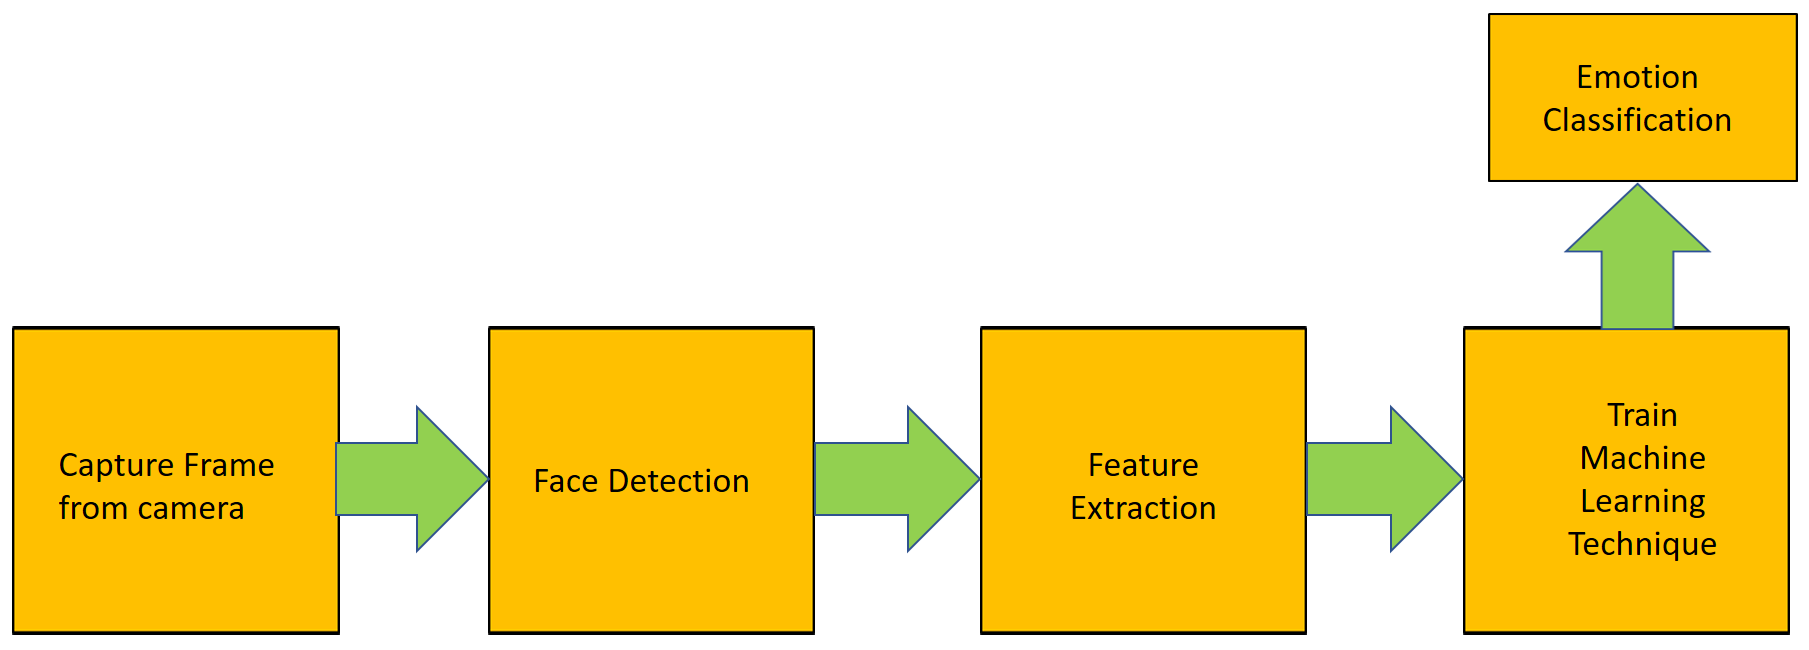
\includegraphics[scale=0.2]{pres1}
  \caption{High-Level View of System}
  \label{fig: highlevel}
\end{figure} 
Looking at Figure ~\ref{fig: highlevel}, the High-level view is explained as:

\begin{itemize}
  \item \textbf{Capture Frame} -- The web camera records a constant stream of video input. The video input consists of a sequence of multiple image frames. The system captures each frame for processing as it is displayed on the video feed.

  \item \textbf{Face Detection} -- Now that we have captured a single frame, we need to check if there is a face present in the frame. This is done using a face detection algorithm. If a face is present in the frame, the location of the face is extracted. The rest of the image is disregarded at this point.

  \item \textbf{Feature Extraction} -- Every emotion displayed facially has it's own set of unique identifying features. By applying feature extraction we are able to represent these features in a way that a computer can understand and process. The feature extraction method is applied to the region of the image that contains the face.

  \item \textbf{Train Machine Learning Technique} -- Machine learning is a method used by computers to learn how to identify patterns in a given set of features. This process is called training. When we train the system, our features are labelled (\textit{Happy, Sad, Angry} etc.). Labelling the features helps guide the computer in the learning process.

  \item \textbf{Emotion Classification} -- When the training is complete, classification helps to test the accuracy of the trained model. At this point the model should be able to identify emotions given unlabelled features.
\end{itemize}

\section{Low-Level View of the System}\label{sec:lowlevel}
The high-level view of the system dives deeper into the details of the components used to implement the system. This is done following the same stages used in the high-level view of the system. In this section we will look at three conceptual low-level views that relate to our system. These views are aligned to the processes followed in image processing, Support Vector Machine model testing \& training and implementing the final system.
\subsection{Low-Level View of Image Processing}

The first low-level view is a visual representation of how the high-level view relates to the image processing techniques discussed in Chapter 3 is presented in Figure~\ref{fig: lowlevel}. 
\begin{figure}[H]
  \centering
  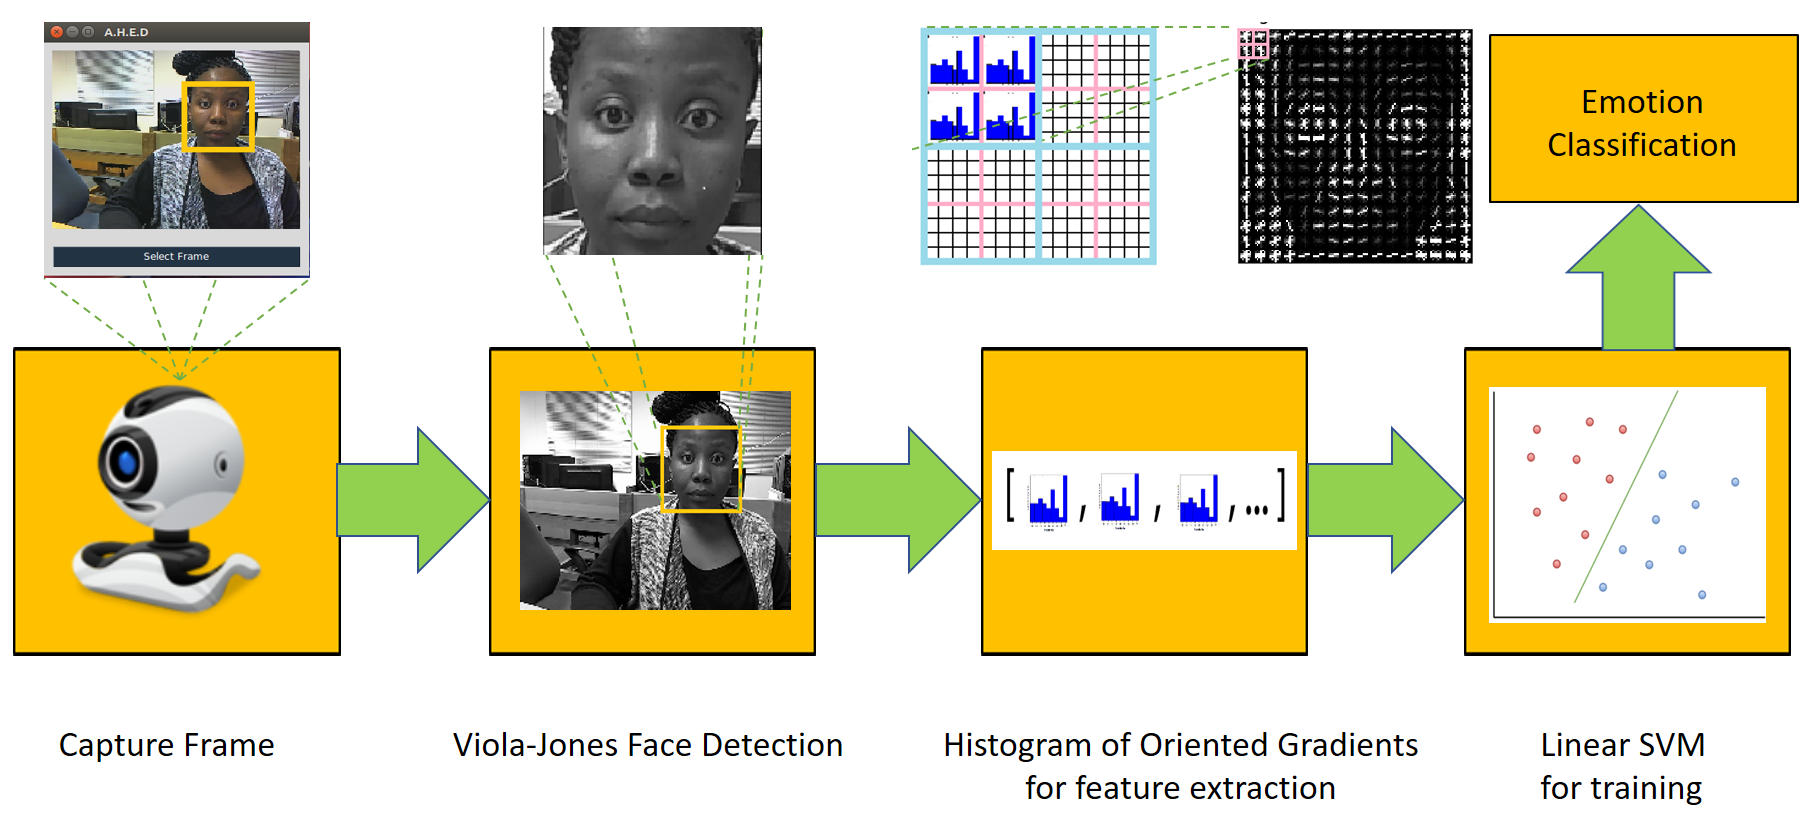
\includegraphics[scale=0.2]{pres2}
  \caption{Low-Level View of Image Processing}
  \label{fig: lowlevel}
\end{figure} 

\subsection{Low-Level View of SVM Model Testing \& Training}

The second low-level view relates to the training and testing of the SVM model used to classify the emotions. Where the `Capture Frame' stage is replaced by `Get Images from Dataset'.
\begin{figure}[H]
  \centering
  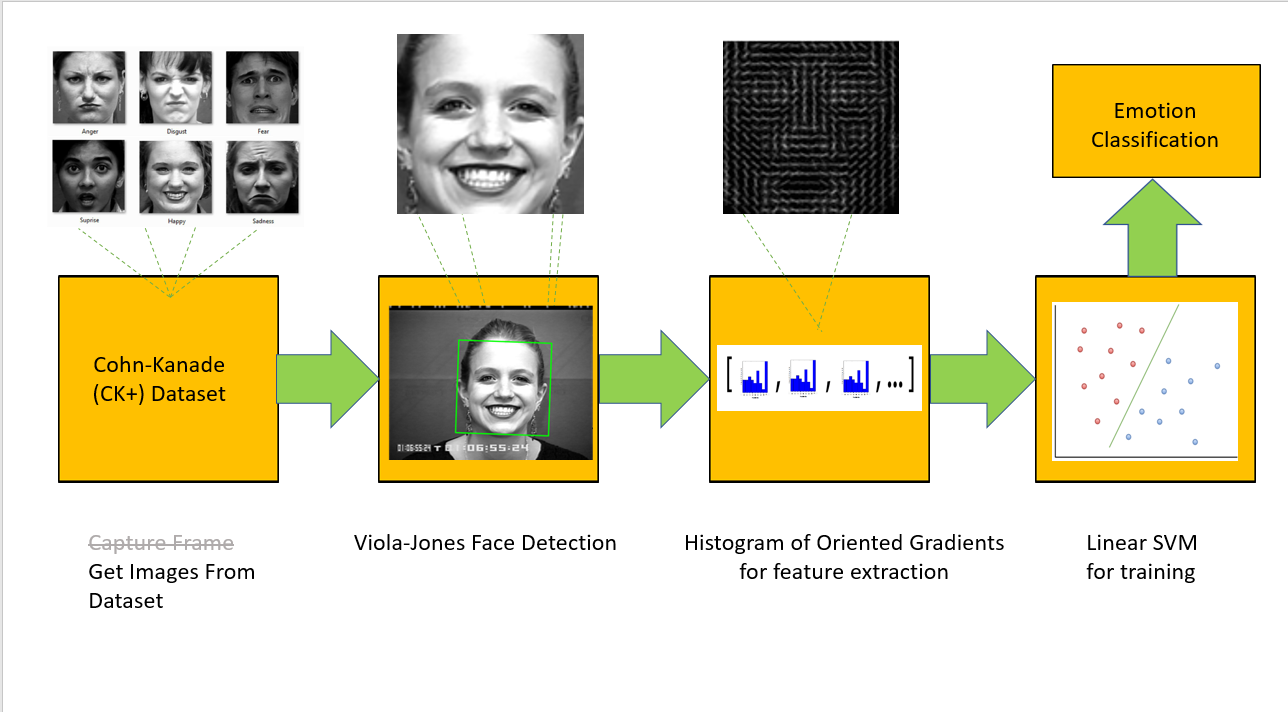
\includegraphics[scale=0.65]{second}
  \caption{Low-Level View of SVM Model Testing \& Training}
  \label{fig: lowlevel2}
\end{figure} 
Looking at Figure~\ref{fig: lowlevel2}, the Low-level view for SVM model testing and training is explained as:

\begin{itemize}
  \item \textbf{Get Images From Dataset} -- The Extended Cohn-Kanade Dataset \citep{ck} is used as data for the training and testing of our SVM model. The images are divided into seven groups, whose labels are: \textit{Angry, Disgust, Fear, Happy, Sadness, Surprise} and \textit{Neutral}. The Table \ref{table:1} provides the total number of images present for each label.

\begin{table}[H]
\centering
\begin{tabular}{ |c||c|}	
	\hline
	\textbf{Emotion Label} & \textbf{N}  \\
	\hline 
	Angry & 45 \\ 
	Disgust & 59 \\ 
	Fear & 25 \\ 
	Happy & 69 \\ 
	Sadness & 28 \\ 
	Surprise & 83 \\  
	Neutral & 35 \\
	\hline  
\end{tabular}
\caption{CK+ Image Labels and Totals}
\label{table:1}
\end{table}

  \item \textbf{Face Detection} -- The Viola-Jones face detection is used to extract the face from each image in the CK+ dataset. The face region of the image is stored as a $56 \times 56$ pixel grayscale image. 
  
  \item \textbf{Feature Extraction} -- The resulting images from the face detection are used as inputs for the Histogram of Oriented Gradients which gives a one-dimensional feature vector for each image. Each image is given a numerical label from 1 to 7 based on the emotion displayed in the image, see Table \ref{table:22} for the labels. The feature vector is stored in the feature dataset with the corresponding numerical emotion label(e.g. [Numerical Label][Feature Vector]). 
\begin{table}[H]
\centering
\begin{tabular}{ |c||c|c|c|c|c|c|c|}
	\hline
	\textbf{Emotion Label}  & Angry & Disgust & Fear & Happy & Neutral & Sadness & Surprise \\ 
	\hline
	\textbf{Numerical Label} & 1 & 2 & 3 & 4 & 5 & 6 & 7   \\ 
	\hline
\end{tabular}   
\caption{Emotions with corresponding Labels for the feature vectors}
\label{table:22}
\end{table}

 The parameters used for the HOG are listed in Table \ref{table:2}.
\begin{table}[H]
\centering
\begin{tabular}{ |c|c|c|}
	\hline
	\textbf{Parameter} & \textbf{Size} & \textbf{Type}  \\
	\hline
	Image & $(56,56)$ & Pixels \\ 
	Cell & $(4,4)$ & Pixels \\ 
	Block & $(3,3)$ & Cells \\ 
	Overlap & $66.66 \%$ & Blocks \\ 
	Bins & $9$ & (0\si{\degree}-180\si{\degree}) Unsigned Gradients\\  
	\hline
	\multicolumn{3}{|c|}{Feature Vector Size: $11664$}\\ 
	\hline
\end{tabular}   
\caption{HOG Parameters}
\label{table:2}
\end{table}

  \item \textbf{Train Machine Learning Technique} -- The machine learning technique used to do the classification for our system is Support Vector Machines. \cite{ck} Used SVMs to test the accuracy of their CK+ dataset due to its proven accuracy with face and facial action detection. An SVM attempts to separate the closest negative and positive points in each class from each other. Once this separation is achieved it makes it easier to separate negative and positive points that are further away from each other, as the similarities in these points are less than those in the points that are closer. The distance between these points is calculated by subtracting the positive and negative points from each other. The positive and negative points closest to each other are considered our support vectors, these help in determining the separating hyperplane. The SVM needs to ensure that the distance between the support vectors is maximized. Figure~\ref{fig: svm} visualizes the concepts discussed.\\

\begin{figure}[H]
  \centering
  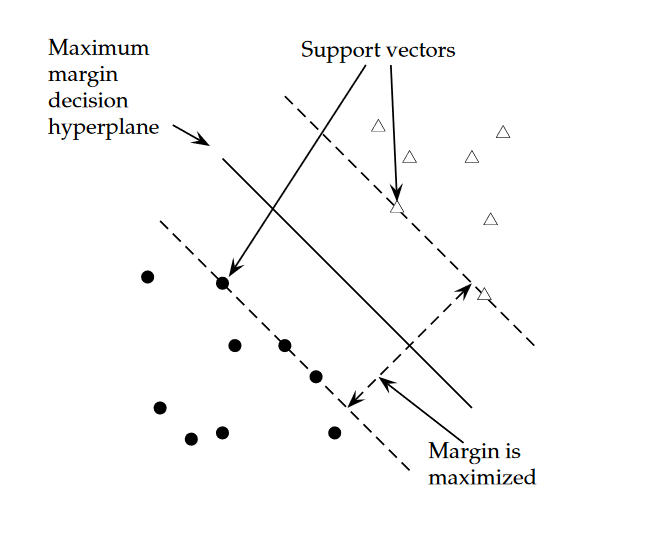
\includegraphics[scale=0.6]{svm}
  \caption{Key Functions of a SVM \cite{stan}}
  \label{fig: svm}
\end{figure} 

\textbf{Cross-Validation} -- The feature dataset compiled after completing the feature extraction is used as input for the SVM. Where the dataset is divided into a training and testing dataset. The percentage of the split is dependent on how well the model performs with each split. A 60\% training and 40\% testing split was used for the SVM. Both these datasets should contain an equal distribution of the emotion labels in each dataset. This step ensures that all labels appear equally in both datasets. The Cross-validation score using a stratified K-fold of 3 is approximately 84\%. Cross-validation measures the overall performance of the SVM model on different training and testing data splits \cite{svm}. This tests the independence of the model to the dataset and helps to prevent overfitting in our model. K-fold cross-validation is done by splitting the dataset into K subsets of equal length. Each subset is then tested on the SVM model of the remaining K-1 subsets. Stratified K-fold cross-validation ensures that the classes are distributed equally in each subset. The training dataset is used as input for training our SVM and creating the SVM model that will be used in our system.\\

\textbf{Grid-Search} -- After optimizing the SVM model with grid-search a Linear Kernel with a C of 1 was used. Grid search helps to find the optimal parameters for the SVM model. Where C determines the extent to which the SVM model should avoid misclassification in the training \cite{svm}. Larger values of C decrease the margin of the hyperplane which aims to increase the accuracy of the training. A smaller value for C increases the margin of the hyperplane, but carries the downside of more misclassified training data points. In \cite{svm} the optimal range for $C = 2^{-5}, 2^{-3}, ..., 2^{15}$. 

\item \textbf{Emotion Classification} -- The testing dataset is used to asses the performance of the the trained SVM model on unseen data. Where the SVM model is given the testing dataset features without the corresponding labels. The results of the SVM model classification are then compared to the original labels to test the accuracy of the SVM model. The SVM model trained for our system has an overall accuracy score of 88.2\%.\\
\item \textbf{Confusion Matrix} -- See Figure~\ref{fig:conf}, a confusion matrix summarises the outcomes of the classification based on the the actual labels of the testing data and those obtain from testing. The values obtained from the confusion matrix help with analyzing the SVM mode. Figure~\ref{fig:conf1} shows the confusion matrix for our SVM model. The diagonal starting at the top-left index till the bottom-right index contains all the true positives/negatives for our SVM model.

\begin{figure}[H]
\centering
\begin{minipage}{.485\textwidth}
  \centering
  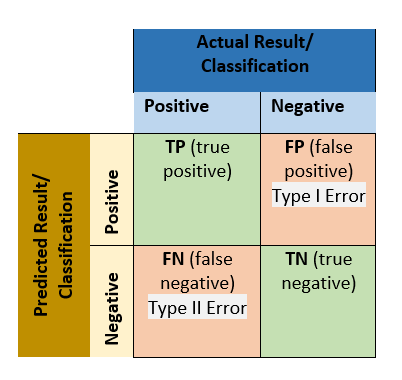
\includegraphics[width=.9\linewidth]{conf}
  \captionof{figure}{Confusion Matrix}
  \label{fig:conf}
\end{minipage}%
\begin{minipage}{.485\textwidth}
  \centering
  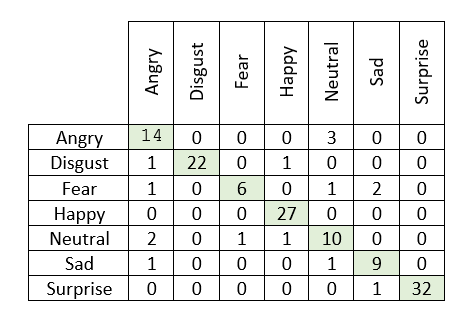
\includegraphics[width=.9\linewidth]{conf1}
  \captionof{figure}{Confusion Matrix of SVM Model Classification}
  \label{fig:conf1}
\end{minipage}
\end{figure}
 
\end{itemize}

\subsection{Low-Level View of Final System}
The third low-level view shows how the process of Automatic Human Emotion Detection is streamlined for user interaction. Where classifications are performed live as the user changes their facial expressions. At this point we use the 'Trained SVM Model' with the HOG parameters from Table \ref{table:2} above.
\begin{figure}[H]
  \centering
  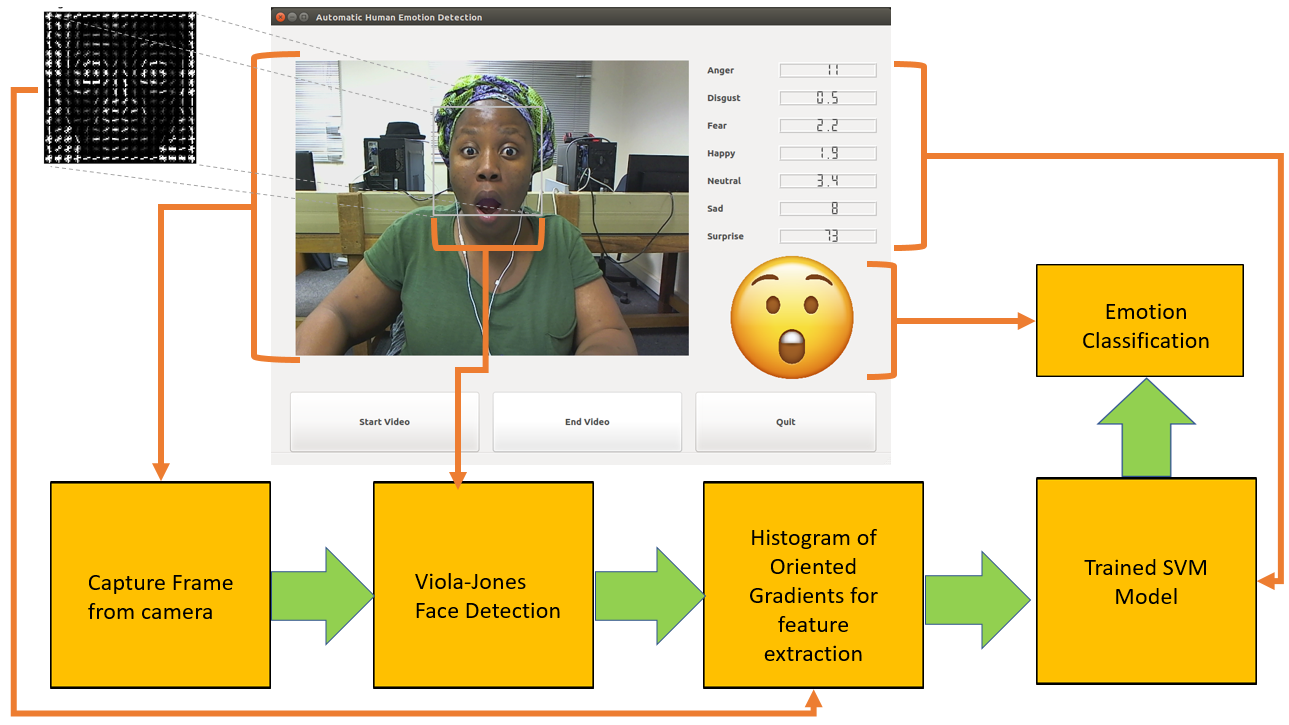
\includegraphics[scale=0.6]{demo}
  \caption{Low-Level View of Final System}
  \label{fig: lowlevel3}
\end{figure} 

\subsection{Optimizing HOG features}
This section covers the different combinations for the HOG parameters that were considered before the values in Table \ref{table:2} were chosen. The HOG implemented from scratch by us is compared to the OpenCV HOG using the Python Sklearn SVM library. All the other parameters remained the same at this point, the dataset had a 60\% training and 40\% testing dataset. The SVM model optimized to a Linear Kernel with a C of 1 for each iteration of the HOG features optimization. Both HOGs maintained a bin size of 9 and 50\% overlap for Block $(2,2)$, with a 66.66\% overlap for Block $(3,3)$.
\begin{table}[H]
\centering
\begin{tabular}{ |c||c|c|}
	\hline
	\multicolumn{3}{|c|}{\textbf{Accuracy of HOG Parameters}}\\
	\hline
	- & \textbf{Cell $(8,8)$ Block $(3,3)$} & \textbf{Cell $(4,4)$ Block $(3,3)$}\\
	\hline
	OpenCV HOG & 86\% & 88.2\% \\
	\hline
	AHED HOG & 77.9\% & 75.7\% \\
	\hline
	& \textbf{Cell $(8,8)$ Block $(2,2)$} & \textbf{Cell $(4,4)$ Block $(2,2)$}\\
	\hline
	OpenCV HOG & 83.8\% & 83.8\% \\
	\hline
	AHED HOG & 77.9\% & 82.3\% \\
	\hline
\end{tabular}
\caption{HOG Optimization}
\label{table:class}
\end{table}
\section{Conclusion}
The Automatic Human Emotion Detection system was implemented entirely using Python. OpenCV is used for the Viola-Jones face detection, Sklearn was used to implement the Histograms of Oriented gradients and the Support Vector Machines. The HOG implementation done from scratch used python numpy arrays and followed the implementation method discussed in Chapter 3. The highest accuracy achieved for the HOG implemented with OpenCV was 88.2\% and 82.3\% with the HOG implemented in this project. 



